\documentclass[12pt,a4paper]{report}
\usepackage[brazil]{babel}
\usepackage[]{algorithm}
\usepackage[]{algorithmic}

\usepackage[style=numeric,backend=biber]{biblatex}
\usepackage[utf8]{inputenc}
\usepackage{kpfonts}
\usepackage[T1]{fontenc}
\usepackage{wrapfig}
\usepackage{graphicx}
\usepackage{enumerate}
\usepackage{subcaption}
\usepackage{float}
\usepackage{caption}
\usepackage{listings}
\usepackage{lipsum}
\usepackage{amsthm}
\usepackage{amssymb}
\usepackage{bm}
\usepackage{color}
\usepackage{afterpage}
\usepackage[inline]{enumitem}
\usepackage{pdflscape}
\usepackage{listingsutf8}
\usepackage{siunitx}
\usepackage{bashful}

\usepackage[margin=1in]{geometry}

\lstset{frame=tb,
  aboveskip=2mm,
  belowskip=2mm,
  showstringspaces=false,
  columns=flexible,
  basicstyle=\footnotesize,,
  numbers=left,
  numbersep=5pt,
  stepnumber=1,
  breaklines=true,
  keepspaces=true,
  breakatwhitespace=true,
  showtabs=false,  
  tabsize=2
}


% Definindo estilo para os códigos
\definecolor{mGreen}{rgb}{0,0.6,0}
\definecolor{mGray}{rgb}{0.5,0.5,0.5}
\definecolor{mPurple}{rgb}{0.58,0,0.82}
\definecolor{dkgreen}{rgb}{0,0.6,0}
\definecolor{backgroundColour}{rgb}{0.97,0.97,0.97}

\lstset{basicstyle=\ttfamily,
    backgroundcolor=\color{backgroundColour},   
    commentstyle=\color{mGreen},
    keywordstyle=\color{magenta},
    numberstyle=\tiny\color{mGray},
    commentstyle=\color{dkgreen},
    stringstyle=\color{mPurple},
    basicstyle=\footnotesize,
    breakatwhitespace=false\textbf{,}         
    breaklines=true,                 
    captionpos=b,                    
    keepspaces=true,                 
    numbers=left,                    
    numbersep=5pt,                  
    showspaces=false,                
    showstringspaces=false,
    showtabs=false,                  
    tabsize=2,
    language=bash
}

\lstdefinestyle{BStyle}{
    backgroundcolor=\color{backgroundColour},  
    showstringspaces=false,
    numbers=none,
    language=bash
}

\pagenumbering{arabic}
\renewcommand{\thesection}{\arabic{section}}

\bibliography{ref}
\renewcommand{\contentsname}{Sumário}{\thispagestyle{empty}}
\renewcommand{\baselinestretch}{1.5} 

\begin{document}

\begin{titlepage}
    \begin{center}
        \vspace*{1cm}
        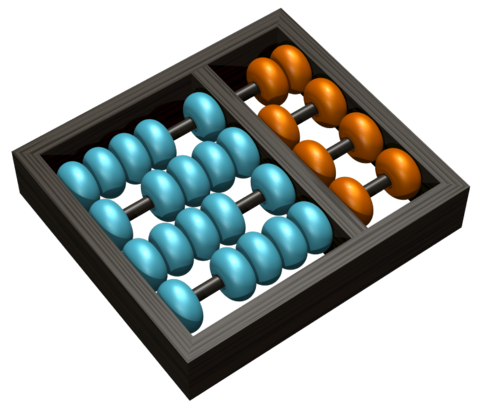
\includegraphics[width=0.25\textwidth]{Logo}\\
        \vspace{1.5cm}
        \Huge
        \textbf{Exercício 1}\\
        \vspace{1.5cm}
        \Large
        \textbf{Aluno}: João Vitor Gonçalves\\
        \textbf{RA}: 176353\\
        \vspace{1.2cm}
        \Large
        Instituto de Computação\\
        Universidade Estadual de Campinas\\
        \vspace{1.5cm}
        Campinas, 23 de Setembro de 2020.
    \end{center}
\end{titlepage}
\tableofcontents
\clearpage

\newcommand{\shellcmd}[1]{\texttt{\footnotesize\# #1}}%estilizando citação de comandos do shell

% \section{Insertion Sort}

% \subsubsection{Pseudocódigo}
% \begin{algorithm}
% \caption{InsertionSort(A)}
% \begin{algorithmic}[1]
%     \STATE $A[0] \longleftarrow -\alpha$
%   \STATE $i \longleftarrow 2 $
%     \FOR {$i$ to $N $} 
%             \STATE $j \longleftarrow i$

%             \WHILE{$A[j] > A[j-1]$} 
%                 \STATE $T \longleftarrow A[j-1]$ 
%                 \STATE $A[j-1] \longleftarrow A[j]$ 
%                 \STATE $A[j] \longleftarrow T$ 
%                 \STATE $j = j -1$
%             \ENDWHILE
%     \ENDFOR
%     \RETURN $A$
%     \end{algorithmic}
% \end{algorithm}



\section{ifconfig}

\subsection{Qual opção deve ser usada para exibir informações sobre todas as interfaces de rede?}

O comando \emph{ifconfig} quando executado sem argumentos, lista as interfaces de rede ativas. eg:

\begin{lstlisting}[language=bash]
$ ifconfig
\end{lstlisting}

\noindent Para mostrar todas as interfaces de rede, ele deve ser executado com a flag \textbf{-a}

\begin{lstlisting}[language=bash]
$ ifconfig -a
br-a10973c7ec6c: flags=4099<UP,BROADCAST,MULTICAST>  mtu 1500
        inet 172.19.0.1  netmask 255.255.0.0  broadcast 172.19.255.255
        ether 02:42:b8:fe:ac:23  txqueuelen 0  (Ethernet)
        RX packets 0  bytes 0 (0.0 B)
        RX errors 0  dropped 0  overruns 0  frame 0
        TX packets 0  bytes 0 (0.0 B)
        TX errors 0  dropped 0 overruns 0  carrier 0  collisions 0

docker0: flags=4099<UP,BROADCAST,MULTICAST>  mtu 1500
        inet 172.17.0.1  netmask 255.255.0.0  broadcast 172.17.255.255
        ether 02:42:2b:e6:81:df  txqueuelen 0  (Ethernet)
        RX packets 0  bytes 0 (0.0 B)
        RX errors 0  dropped 0  overruns 0  frame 0
        TX packets 0  bytes 0 (0.0 B)
        TX errors 0  dropped 0 overruns 0  carrier 0  collisions 0

eno1: flags=4163<UP,BROADCAST,RUNNING,MULTICAST>  mtu 1500
        inet 192.168.100.128  netmask 255.255.255.0  broadcast 192.168.100.255
        inet6 fe80::6799:e59a:3a29:3c46  prefixlen 64  scopeid 0x20<link>
        ether 00:d8:61:6f:ea:50  txqueuelen 1000  (Ethernet)
        RX packets 5253629  bytes 6151206386 (6.1 GB)
        RX errors 0  dropped 0  overruns 0  frame 0
        TX packets 1812540  bytes 191417863 (191.4 MB)
        TX errors 0  dropped 0 overruns 0  carrier 0  collisions 0
        device interrupt 16  memory 0xa4200000-a4220000  

lo: flags=73<UP,LOOPBACK,RUNNING>  mtu 65536
        inet 127.0.0.1  netmask 255.0.0.0
        inet6 ::1  prefixlen 128  scopeid 0x10<host>
        loop  txqueuelen 1000  (Local Loopback)
        RX packets 808745  bytes 648198978 (648.1 MB)
        RX errors 0  dropped 0  overruns 0  frame 0
        TX packets 808745  bytes 648198978 (648.1 MB)
        TX errors 0  dropped 0 overruns 0  carrier 0  collisions 0    
\end{lstlisting}

\noindent Assim serão exibidas todas as interfaces, mesmo as desativadas.

\subsection{O que deve ser feito para exibir somente informações de uma interface específica?}

Para exibir informações de somente uma interface específica, o seu nome deve ser passado como um argumento para o comando:

\begin{lstlisting}[language=bash]
$ ifconfig br-a10973c7ec6c
br-a10973c7ec6c: flags=4099<UP,BROADCAST,MULTICAST>  mtu 1500
        inet 172.19.0.1  netmask 255.255.0.0  broadcast 172.19.255.255
        ether 02:42:b8:fe:ac:23  txqueuelen 0  (Ethernet)
        RX packets 0  bytes 0 (0.0 B)
        RX errors 0  dropped 0  overruns 0  frame 0
        TX packets 0  bytes 0 (0.0 B)
        TX errors 0  dropped 0 overruns 0  carrier 0  collisions 0
\end{lstlisting}

\section{nslookup}
\subsection{Quais são os endereços IP do host www.unicamp.br?}
\subsection{Há alguma vantagem em haver mais de um endereço IP?}

\section{traceroute}
\subsection{Quantos roteadores estão entre a sua estação e o host www.amazon.com? Pelos nomes dos roteadores, quantos deles estão localizados no Brasil?}

Executando o comando \emph{traceroute} para o endereço \emph{www.amazon.com} obtemos: 

\begin{lstlisting}[language=bash]
        $ traceroute www.amazon.com   
        traceroute to www.amazon.com (13.33.130.223), 30 hops max, 60 byte packets
         1  _gateway (192.168.100.1)  0.390 ms  0.344 ms  0.288 ms
         2  192.168.0.1 (192.168.0.1)  1.439 ms  1.494 ms  1.341 ms
         3  10.21.0.1 (10.21.0.1)  14.750 ms  8.691 ms  14.799 ms
         4  c94c1001.virtua.com.br (201.76.16.1)  17.870 ms  17.867 ms  18.191 ms
         5  embratel-G0-5-3-2-tacc01.cas.embratel.net.br (200.174.243.53)  20.587 ms embratel-T0-3-0-0-uacc02.cas.embratel.net.br (189.16.179.53)  22.126 ms  22.086 ms
         6  ebt-H0-7-0-3-tcore01.cas.embratel.net.br (200.244.213.103)  33.239 ms ebt-H0-4-0-0-tcore01.cas.embratel.net.br (200.244.212.61)  36.143 ms ebt-H0-7-0-3-tcore01.cas.embratel.net.br (200.244.213.103)  24.095 ms
         7  ebt-B1191-tcore01.spo.embratel.net.br (200.230.252.130)  35.167 ms  33.017 ms  24.929 ms
         8  ebt-B2111-tcore01.rjo.embratel.net.br (200.230.251.1)  37.181 ms  31.957 ms  33.497 ms
         9  ebt-H0-2-0-1-uacc04.rjoen.embratel.net.br (200.244.211.210)  30.454 ms  30.465 ms ebt-H0-7-0-1-uacc04.rjoen.embratel.net.br (200.244.211.214)  30.384 ms
        10  peer-B55-uacc04.rjoen.embratel.net.br (189.87.140.110)  30.038 ms  28.433 ms  28.439 ms
        11  52.93.67.58 (52.93.67.58)  27.497 ms peer-B55-uacc04.rjoen.embratel.net.br (189.87.140.110)  26.865 ms  21.708 ms
        12  52.93.67.197 (52.93.67.197)  30.382 ms 52.93.67.199 (52.93.67.199)  30.470 ms *
        13  * * *
        ...
\end{lstlisting}

Cosiderando o roteador \emph{gateway} local, temos um total de 12 roteadores entre a minha interface de rede e o host \emph{www.amazon.com}.

Podemos observar que até o roteador de número \textbf{10}, os roteadores estão localizados no Brasil, uma vez que possuem nomes relacionados à Embratel ou à Net Virtua.
E a partir do roteador \textbf{11}, podemos observar por meio do comando \emph{whois} que os endereços dos roteadores \emph{11} e \emph{12} são pertencentes à \emph{amazon}.

\begin{lstlisting}[language=bash]
        $whois 52.93.67.58
        ... 
        OrgName:        Amazon Technologies Inc.
        OrgId:          AT-88-Z
        Address:        410 Terry Ave N.
        City:           Seattle
        StateProv:      WA
        PostalCode:     98109
        Country:        US
        ...
\end{lstlisting}


\begin{lstlisting}[language=bash]
        $whois 52.93.67.197
        ... 
        OrgName:        Amazon Technologies Inc.
        OrgId:          AT-88-Z
        Address:        410 Terry Ave N.
        City:           Seattle
        StateProv:      WA
        PostalCode:     98109
        Country:        US
        ...
\end{lstlisting}





\section{telnet}
\subsection{É possível conectar-se com este comando em um servidor HTTP? Se sim, como deve-se executar o comando para conectar-se no host www.amazon.com na porta padrão do HTTP?}
\subsection{Caso não haja um servidor escutando na porta passada pelo comando telnet, o que ocorre? Justifique.}
\subsection{A qual a camada da rede o telnet pertence?}

\section{Acesse o site da DAC (https://www.dac.unicamp.br/) e, em paralelo em um terminal, verifique a saída do comando netstat. Quais são as informações fornecidas a respeito da conexão ao site da DAC?}

\section{TCPDUMP}
\subsection{Utilizando o TCPDUMP corretamente com os filtros é possível somente capturar o tráfego HTTPS? Se sim, execute o comando junto com os filtros e anexe uma figura que comprove sua resposta no relatório. Se sua resposta foi não, então justifique-a.}
\subsection{Utilizando o comando TCPDUMP seguido dos parâmetros corretos imprima somente os pacotes superiores a 64 bits. Indique qual foi a sequência de comandos utilizada.}
\subsection{Utilizando o TCPDUMP seguido de filtros, imprima somente os resultados que tiverem a flag ‘ACK’. Insira o comando seguido dos filtros e uma figura no seu relatório para comprovar o sucesso.}

\section{Wireshark}


\subsection{Comparado às demais ferramentas apresentadas na aula de MC833 descreva quais são principais diferenças e vantagens de usar o Wireshark? Escolha pelo menos uma ferramenta/sniffer e elabore uma tabela comparativa para responder a questão.}

\subsection{Em uma rede com vários processos acontecendo ao mesmo tempo é possível gerenciar de forma isolada um único processo específico na rede utilizando ferramentas/sniffers apresentados nesta disciplina? Se sim, quais ferramentas e/ou sniffers você usaria? Justifique sua resposta. (OBS: Não é necessário apresentar comandos ou prints)}


\end{document}